\documentclass{article}
\usepackage[utf8]{inputenc}
\usepackage{caption}
\usepackage{amsmath}
\usepackage{amssymb}
\usepackage{mathtools}
\usepackage{multicol}
\usepackage{graphicx}
\usepackage{wrapfig}
\usepackage{float}
\usepackage[makeroom]{cancel}
\usepackage{mhchem}
\usepackage{pst-plot}

\graphicspath{ {../images/} }

\renewcommand{\baselinestretch}{1.5} % line spacing
\newcommand{\fline}{\par\noindent\rule{\textwidth}{0.1pt}} % horizontal line (wide)

\title{Unit 2 Kinetics\\Lesson 3 Rate Expressions and Order}
\author{Peter Zhang}

\begin{document}

\maketitle
\newpage
\tableofcontents
\newpage

% lesson 3

\section{Order}
\subsection{0th Order}
Zero order reactions are flat

\begin{figure}[H]
\centering
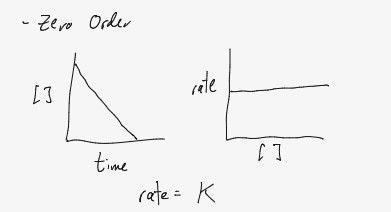
\includegraphics[width=200pt]{2.3fig1.jpg}
\captionof{figure}{Linear for 0th Order}
\end{figure}

Insert linear line y = (-x + 1) diagram (first order) | And y = 4

\subsection{1st Order}
First order reactions are linear
\begin{figure}[H]
\centering
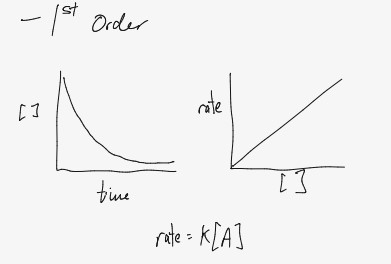
\includegraphics[width=200pt]{2.3fig2.jpg}
\captionof{figure}{Linear for 1st Order}
\end{figure}


$$rate = k\ce{[A]}^1$$

\subsection{2nd Order}
Second order reactions are not linear (they are curved)

\begin{figure}[H]
\centering
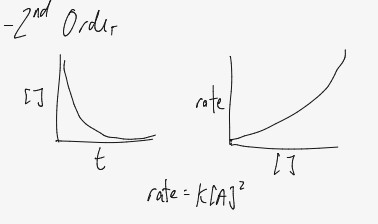
\includegraphics[width=300pt]{2.3fig3.jpg}
\captionof{figure}{Linear for 2nd Order}
\end{figure}

$$rate = k\ce{[A]}^2$$



\begin{itemize}
\item If a change in [c] has no effect it is zero order
\item If a change in [c] is proportional to chnages in rate,  $\rightarrow 1^{st}$ order\\If doubling [c], there should be a doubling in rate (proportional)
\item If a change in [c] leads to the square of that change in rate, it is $2^{nd}$ order\\If doubling [c], the rate should increase by 4
\end{itemize}


\pagebreak
\subsection{Example}

\begin{center}
\begin{tabular}{|c|c|c|c|c|}
\hline
Experiment & [A] & [B] & [C] & Rate \\
\hline \hline
1 & 0.1 & 0.1 & 0.1 & $6.2*10^{-4}$\\
\hline
2 & 0.1 & 0.2 & 0.1 & $1.2*10^{-3}$\\
\hline
3 & 0.1 & 0.1 & 0.2 & $6.2*10^{-4}$\\
\hline
4 & 0.2 & 0.1 & 0.2 & $2.5*10^{-3}$\\
\hline
\end{tabular}
\end{center}

\begin{align*}
[B] & = \frac{1.2*10^{-3}}{6.2*10^{-4}}\ ([2]/[3])\\
&= 2
\end{align*}

[B] is $1^{st}$ order

Following general formula outline: -- $[X] = \frac{[Ex4]}{[Ex1]}$ (The one where we double [A] and have normal [A]. This formula gives:

[A] = 4, $\therefore$ [A] is $2^{nd}$ order.\\
And since [C] = 1, $\therefore$ [C] is order 0 (bc the change is 0)

\begin{figure}[H]
\centering
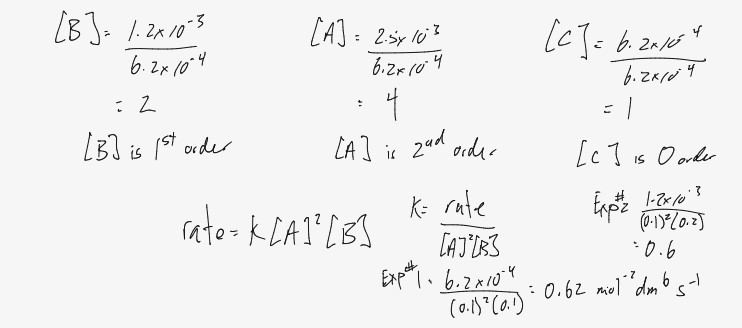
\includegraphics[width=\textwidth]{2.3eq.jpg}
\captionof{figure}{Solving for each concentration}
\end{figure}


\pagebreak
\section{Molecularity}
\begin{itemize}
\item Unimolecular (\# of elements = 1)
\item Bimolecular (\# of elements = 2)
\item Termolecular (\# of elementrs = 3)
\end{itemize}

\subsection{Example}
Ex: \ce{2A + B + C -> 3D + E}\\Assume A is $2^{nd}$ order, B is 0, and C is $1^{st}$ order.

The idea is if AC exists, we want to cancel it out: (this means we need to make another intermediate step)

\begin{enumerate}
\item \ce{A + C -> D + AC} (the slow reaction)
\item \ce{AC + B -> D + E} 
\item \ce{A -> D}
\end{enumerate}
Add them together\\\ce{2A + B + C -> 3D + E}

The (slow) reaction is slow. This means that whatever changes here affects everything else. The slower reaction has the \textbf{BIGGEST} impact on the other equation. 

The intermediate is usually created as a byproduct from the first equation or initial or (slow) reaction. Then \textbf{USUALLY THE INTERMEDIATE does not impact the \underline{rate}}. There are exceptions to this rule.\\
If intermediates are used in the final reaction (equation), then intermediates do effect the rate.


\section{Fast and Slow Reactions}
\subsection{Slow Reactions}
The slow reactions are considered slow because they form intermediate products. 
\subsection{Fast Reactions}
They are considered fast because they the intermediate products quickly form into the products









\end{document}